\documentclass[letter]{article}

\usepackage[english]{babel}
\usepackage[utf8]{inputenc}
\usepackage{amsmath}
\usepackage[colorinlistoftodos]{todonotes}
\usepackage{makecell}
\usepackage{multirow}
\usepackage{caption}
\usepackage{subcaption}
\usepackage{graphicx}
\usepackage{hyperref}
\usepackage{float}
\usepackage[all]{hypcap}
\usepackage[space]{grffile}
\usepackage{enumitem}
\usepackage{bm}
\usepackage{bbm}
\usepackage{algorithm}
\usepackage{algorithmic}
\usepackage{nccmath, mathtools}
\usepackage{amsthm,amssymb}
\usepackage{listings}

\newlist{questions}{enumerate}{1}
\setlist[questions, 1]{label = \arabic*}
\newlist{bonus}{enumerate}{1}
\setlist[bonus, 1]{label = Bonus \arabic*}

\definecolor{mygreen}{rgb}{0,0.6,0}
\definecolor{mygray}{rgb}{0.5,0.5,0.5}
\definecolor{mymauve}{rgb}{0.58,0,0.82}

\lstset{ 
	backgroundcolor=\color{white},   % choose the background color; you must add \usepackage{color} or \usepackage{xcolor}; should come as last argument
	basicstyle=\footnotesize,        % the size of the fonts that are used for the code
	breakatwhitespace=false,         % sets if automatic breaks should only happen at whitespace
	breaklines=true,                 % sets automatic line breaking
	captionpos=b,                    % sets the caption-position to bottom
	commentstyle=\color{mygreen},    % comment style
	deletekeywords={...},            % if you want to delete keywords from the given language
	escapeinside={\%*}{*)},          % if you want to add LaTeX within your code
	extendedchars=true,              % lets you use non-ASCII characters; for 8-bits encodings only, does not work with UTF-8
	frame=single,	                   % adds a frame around the code
	keepspaces=true,                 % keeps spaces in text, useful for keeping indentation of code (possibly needs columns=flexible)
	keywordstyle=\color{blue},       % keyword style
	language=Octave,                 % the language of the code
	morekeywords={*,...},            % if you want to add more keywords to the set
	numbers=left,                    % where to put the line-numbers; possible values are (none, left, right)
	numbersep=5pt,                   % how far the line-numbers are from the code
	numberstyle=\tiny\color{mygray}, % the style that is used for the line-numbers
	rulecolor=\color{black},         % if not set, the frame-color may be changed on line-breaks within not-black text (e.g. comments (green here))
	showspaces=false,                % show spaces everywhere adding particular underscores; it overrides 'showstringspaces'
	showstringspaces=false,          % underline spaces within strings only
	showtabs=false,                  % show tabs within strings adding particular underscores
	stepnumber=2,                    % the step between two line-numbers. If it's 1, each line will be numbered
	stringstyle=\color{mymauve},     % string literal style
	tabsize=2,	                   % sets default tabsize to 2 spaces
	title=\lstname                   % show the filename of files included with \lstinputlisting; also try caption instead of title
}

% Adjust margins
\addtolength{\oddsidemargin}{-0.75in}
\addtolength{\evensidemargin}{-0.75in}
\addtolength{\textwidth}{1.5in}
\addtolength{\topmargin}{-.5in}
\addtolength{\textheight}{1.5in}
\setlength\parindent{0pt}
\setlength{\parskip}{5pt}

\title{CS 520: Assignment 4 - Colorization}
\author{Haoyang Zhang, Han Wu, Shengjie Li, Zhichao Xu}
\date{December 15, 2018}

\begin{document}
\maketitle

\section{Introduction, group members and division of workload}
\label{sec:Introduction}

In this group project, we implemented a image colorizer which can generate satisfying color images given grayscale images. \\
\begin{tabular}{| p{2.5cm} | p{\textwidth -3.5cm} |}
	\hline
	\makecell[c]{Name \\ RUID} & Workload \\
	\hline
	\makecell[c]{Haoyang Zhang \\ 188008687} & {Implemented a toy CNN based on numpy. Wrote Usage.html and HowToBuildACNN.html which are two documents about the toy CNN. Wrote part of the report. Analyzed the performance of this model on images belonging to some classes that have never been trained before.} \\
	\hline
	\makecell[c]{Han Wu \\ 189008460} & {Wrote part of the report and participated in the discussion. Analyzed the outcome of our colorizer.} \\
	\hline
	\makecell[c]{Shengjie Li \\ 188008047} & {Implemented the colorizer. Trained the model. Wrote part of the report. Finished the format design of the report using \LaTeX. } \\
	\hline
	\makecell[c]{Zhichao Xu \\ 188008912} & {Wrote part of the report. Came up with the original structure of network.} \\
	\hline
\end{tabular}


\section{The Problem}
\label{sec:The Problem}
\begin{itemize}
	\item {\textbf{Representing the Process:}   } 
	\begin{enumerate}
		\item {\textbf{How can you represent the coloring process in a way that a computer can handle?}}
		\par{A color image can be interpreted as an array with 3 channels -- channel R,  channel G, channel B. A grayscale image can be interpreted as a color image being compressed to having only one channel gray, by the formula $ Gray(r, g, b) = 0.21r + 0.72g + 0.07b $. So the coloring process can be seen as: given a one-channel image, produce a three-channel image. To achieve this, we are using a convolutional autoencoder -- An autoencoder with convolutional layers in its encoding part and deconvolutional layers in its decoding part.}
		\item {\textbf{What spaces are you mapping between? What maps do you want to consider?} Note that mapping
			from a single grayscale value gray to a corresponding color (r, g, b) on a pixel by pixel basis, you do not have
			enough information in a single gray value to reconstruct the correct color (usually).}
		\par{Every image of the input is a $ 3 \times 32 \times 32 $ numpy array -- RGB values of every pixel. Each RGB value is between [0, 255]. We will first pre-process the data, get the grayscale of the images, standardize the value, make every image to be a $ 1 \times 32 \times 32 $ numpy array with values between [0, 1]. }
		\par{Because we are using tanh as our activation function. So the ouput of the network is a $ 3 \times 32 \times 32 $ array with RGB channels and values between [-1, 1]. We scale it between [0, 1] and use this value to calculate the loss. If we are going to plot the results, we can simply multiply every value by 255.}
		\par{Because of the dense layers, each output pixel whose space size is $ 3 \times 256 \times 1 \times 1 $ is maped from the whole input graph, whose space size is $ 1 \times 256 \times 32 \times 32 $}
	\end{enumerate}
	\item {\textbf{Data:}} 
	\begin{enumerate}
		\item {\textbf{Where are you getting your data from to train/build your model?}}
		\par{We are using the \href{http://www.cs.toronto.edu/~kriz/cifar.html}{The CIFAR-10 dataset}.}
		\par{This dataset consists of 60,000 $ 32\times32 $ colour images in 10 classes, with 6,000 images per class. There are 50,000 training images and 10,000 test images in total. The dataset is divided into five training batches and one test batch, each with 10,000 images. The test batch contains exactly 1,000 randomly-selected images from each class. }
		\begin{figure}[H]
			\centering
			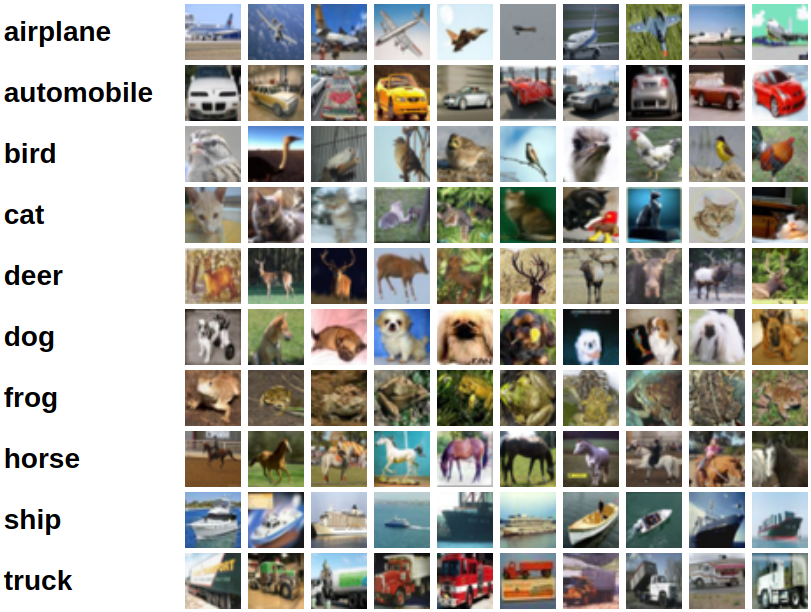
\includegraphics[width=0.7\textwidth]{figs/fig-2.png}
			\caption{The CIFAR-10 dataset}
		\end{figure}
	
		\item {\textbf{What kind of pre-processing might you consider doing?}}
		\par{Each training batch is a $ 10000\times3072 $ numpy array. Each row of the array stores a $ 32\times32 $ colour image. The first 1024 entries contain the red channel values, the next 1024 the green, and the final 1024 the blue. The value of each channel is between $ [0, 255] $. We are going to scale the RGB channel from $ [0, 255] $ to $ [0, 1] $. By standardizing the data, we could train faster and reduce the chance of getting stuck in a local optima.}
	\end{enumerate}
	\item {\textbf{Our Model:}} 
	\par{Our model is an basically autoencoder with convolutional layers in the encoding part and deconvolutional layers in the decoding part.}
	\begin{figure}[H]
		\centering
		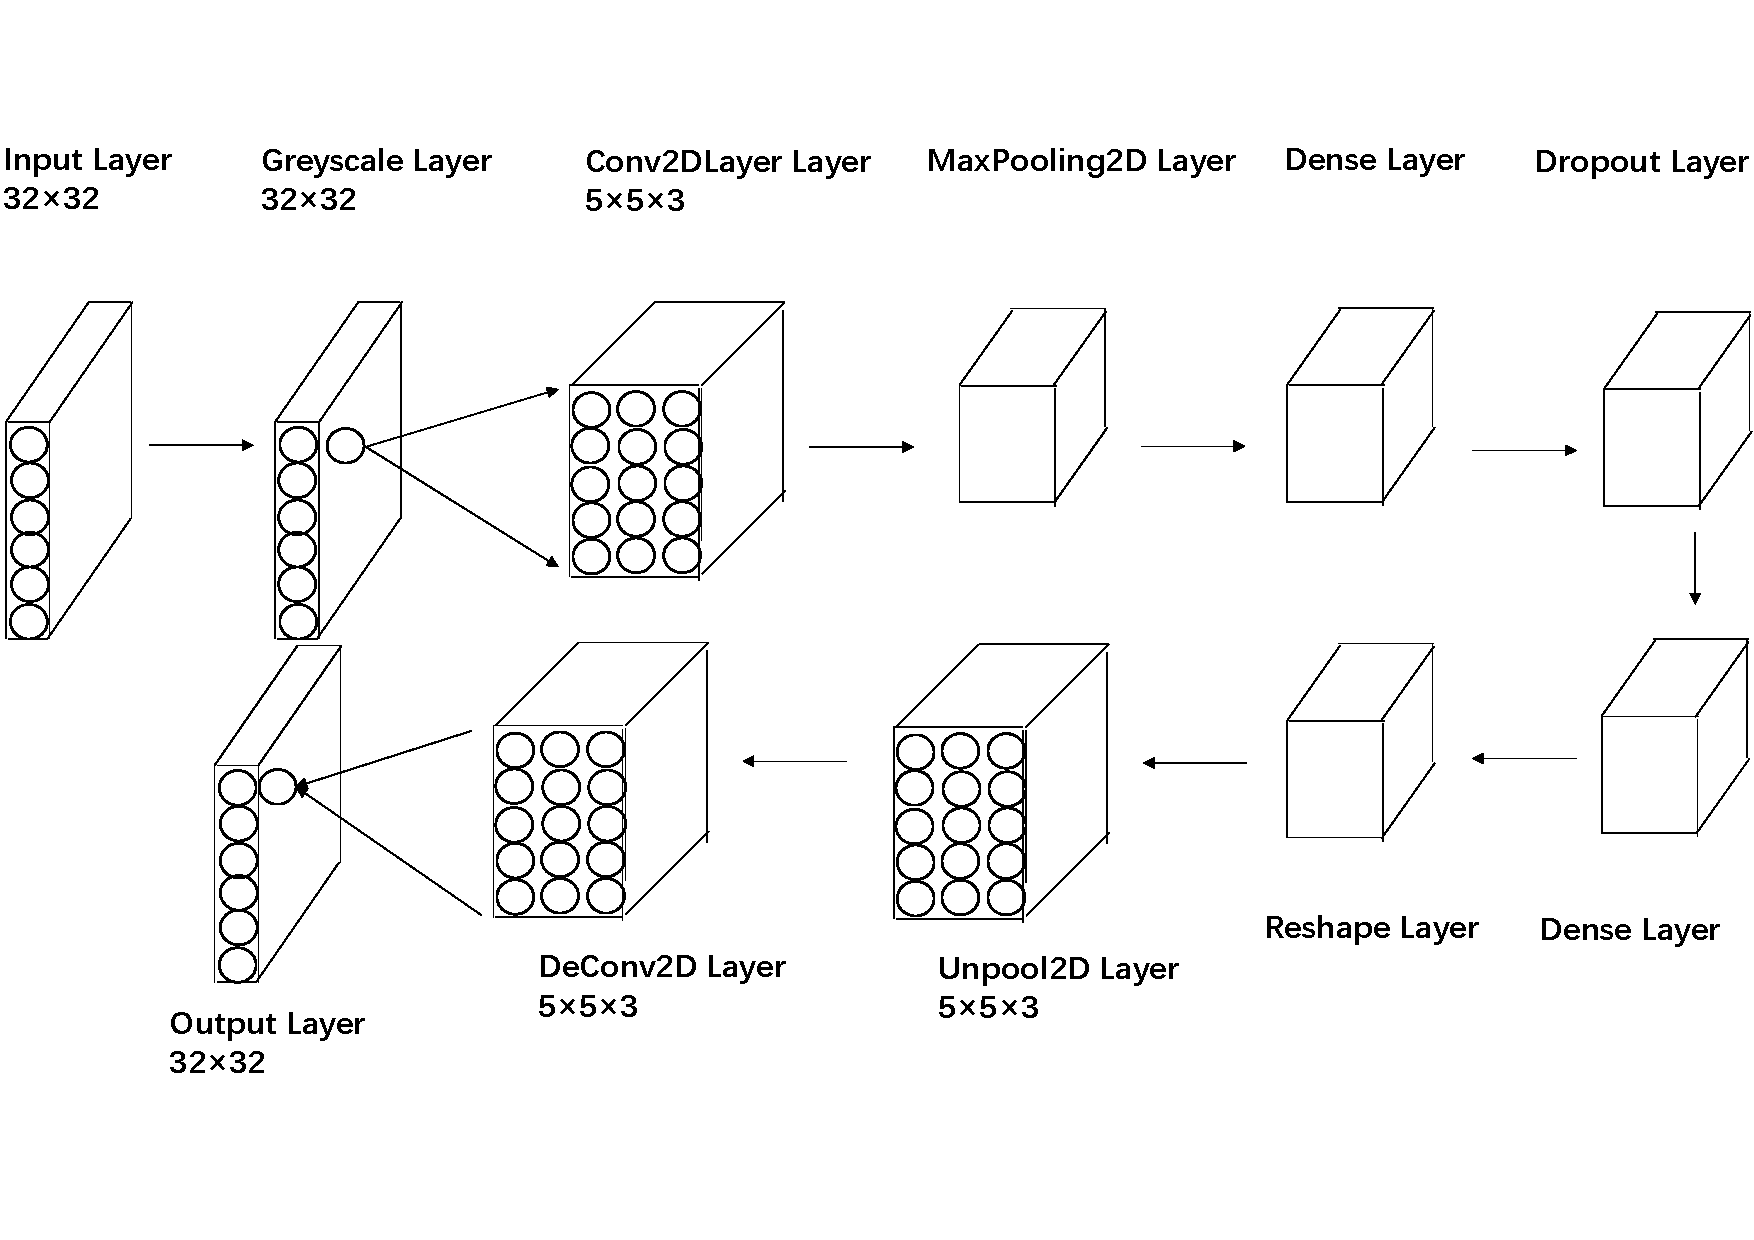
\includegraphics[width=\textwidth]{figs/structure.pdf}
		\caption{Structure of our model}
	\end{figure}
	\begin{enumerate}
		\item {\textbf{Input layer:} uses 4d-tensor to represent the input image.}
		\item {\textbf{Grayscale layer:} calculates the grayscale of the input colored image.}
		\item {\textbf{Convolutional layer:} in this layer we are using a filter of size $ 5\times5 $. During the forward pass, we convolute each filter across the width and height of the input volume and compute dot products between the entries of the filter and the input at any position. In this process, we will produce a 2-d activation map that gives the responses of that filter at every spatial position. Intuitively, the network will learn filters that activate when they see some type of visual features, such as an edge of some orientation or a blotch of some color on the first layer, or eventually some wheel-like patterns on higher layers of the network. We will stack these activation maps along the depth dimension and produce the output volume.}
		\item {\textbf{Max Pooling layer:} this function of this layer is, progressively reducing the spatial size of the representation to reduce the amount, if parameters and computation in the network, and hence to also control overfitting. This layer operates independently on every depth slice of the input and resizes it spatially, using the MAX operation. The window size of this pooling layer is $ 2 \times 2 $.}
		\item {\textbf{Dense layer:} in this layer the neurons have full connections to all activations in the previous layer. Their activations can hence be computed with a matrix multiplication followed by a bias offset.}
		\item {\textbf{Dropout layer:} this layer is a regularizer that randomly sets input values to zero with a probability of 30\%. It is used to prevent overfitting.}
		\item {\textbf{Dense layer:} another fully connected layer.}
		\item {\textbf{Reshape + Max Unpooling layer:} first the reshape layer reshape the data, then the max unpooling layer performs unpooling over the last two dimensions of a 4D tensor. This layer is essential if we want to reconstruct the image.}
		\item {\textbf{Deconvolutional layer:} This layer is used for upsampling (backwards strided convolution). It changes the shape from $ 100 \times 32 \times 32 $ to $ 3 \times 32 \times 32 $ which is the shape we want for an image. It can coarse outputs to dense pixels by interpolation. In-network upsampling is fast and effective for learning dense prediction.}
		\item {\textbf{Reshape + Output layer:} this layer reshapes the network and outputs the generated image.}
	\end{enumerate}
	\item {\textbf{Evaluating the Model:}} 
	\begin{enumerate}
		\item {\textbf{Given a model for moving from grayscale images to color images (whatever spaces you are mapping between), how can you evaluate how good your model is?}}
		\par{For the evaluation part, we used the squared loss as the criteria. \[ \mathcal{L} = || output - input ||^2 \] When the loss is small enough, we can know our model is performing good.}
		\item {\textbf{How can you assess the error of your model (hopefully in a way that can be learned from)? }}
		\begin{itemize}
			\item {From the numerical perspective, the mean squared validation loss is, the better the model is performing. }
			\item {From the perceptual perspective, the closer the color is to the original picture, the better the model is performing.}
		\end{itemize}
	\end{enumerate}
	\item {\textbf{Training the Model:}} 
	\begin{enumerate}
		\item{Representing the problem is one thing, but can you train your model in a computationally tractable manner?}
		\par{It is actually quite easy to train our model because of the small size of the input. Generally, for each iteration, we would need to train for 40 seconds using a GTX 1070ti, for 25 seconds using a GTX 1080ti. We could achieve a good result in less than 100 iterations of training most of the time.}
		\item{What algorithms did you draw on?}
		\par{We are using Stochastic Gradient Descent algorithm with Nesterov momentum to accelerate the training process, and we are using back propagation to update the gradient.}
		\item{How did you determine convergence?}
		\par{We validate the model and print out the validation loss every 10 iterations. When the validation loss stabilizes and even starts to rise, we stop our training and call it a convergence.}
		\item{How did you avoid overfitting?}
		\par{We are using Max Pooling layers and Dropout Layers in our model to prevent overfitting.}
		\begin{itemize}
			\item {Max pooling is basically selecting a subset of features, so we are less likely to be always training on false patterns.}
			\item {Dropout layers randomly drop some components of our neural network with some probability, which actually creates a different network. Thus after we finished the training, we actually have an ensemble of models. The probability is typically 50\%, but after our experiments, we found 30\% is better.}
		\end{itemize}
	\end{enumerate}
	\item {\textbf{Assessing the Final Project:}} 
	\begin{enumerate}
		\item {How good is your final program, and how can you determine that? How
			did you validate it?}
		\begin{figure}[H]
			\centering
			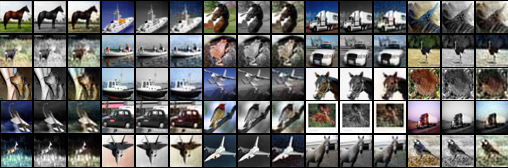
\includegraphics[width=\textwidth]{figs/fig-5.png}
			\caption{Some results}
			\label{fig-5}
		\end{figure}
		\par{Our final model is satisfying as Fig \ref{fig-5} shows. For every three images, they are respectively `the original image' - `grayscale image' - `image colorized by our program'.}
		\par{We use our validation dataset to calculate the validation loss. The validation loss of our final model achieved 20.928495, which is reasonable to us. }
		\item {What is your program good at, and what could use improvement?}
		\par{Our program is performing very good on colorizing animals and vehicles if they are not blue or red. When it comes to images with blue and red colors, our program could totally mess up.}
		\item {Do your program's mistakes `make sense'?}
		\begin{figure}[H]
			\centering
			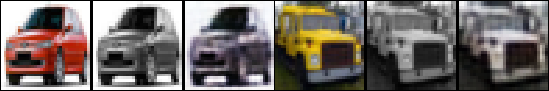
\includegraphics[width=0.7\textwidth]{figs/fig-3.png}
			\caption{Some results}
			\label{fig-3}
		\end{figure}
		\par{The colorizer can totally mess up blue and red or white and yellow as Fig \ref{fig-3} shows. But to be honest, we cannot tell the color of the car by just looking at its grayscale image. We think this kind of mistakes are quite resonable.}
		\item {What happens if you try to color images unlike anything the program was trained on?}
		\begin{figure}[H]
			\centering
			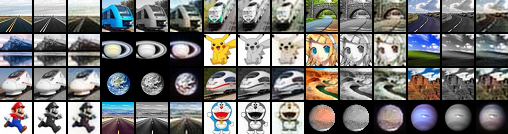
\includegraphics[width=\textwidth]{figs/untrained.png}
			\caption{Some results}
			\label{untrained}
		\end{figure}
		\par{Our dataset contains images from 10 classes -- airplane, automobile, bird, cat, deer, dog, frog, horse, ship, truck. Thus, to verify the performance of this question, we chose a total of 20 images with 5 classes -- Roads, Planets, Trains, Landscapes and Anime Characters. }
		\par{The average loss of all 5 above classes is 60.927757, which is a lot higher compared with a loss of about 20 while validating on trained classes.}
		\begin{itemize}
			\item {For Roads, it performs not bad because a grayscale picture of roads still provides lots of information: roads are dark, lines are light, and sky is nearly white. And since we have trained many car and truck pictures, which contains some roads. It is not suppressing that it performs well.}
			\item {For Trains, some colorized pictures are not that bad compared with the original ones, except that sometimes it colors the train body with a different color. It is reasonable that a train can be either blue or dark yellow. Since there are some similarities between trucks and trains. We can conclude our model have sort of ability of generalizing.}
			\item {Planets are nightmare, but how could we know a planet is red, blue or any other color? They are all round and with nearly the same gray scale.}
			\item {Many mistakes are made when it tries to color images of landscape, but an interesting thing is that it knows all mountains should color brown. Though some mountains are not brown. Nevertheless, it seems have sort of idea of ``Mountains''.}
			\item {Our program failed on all images of Anime Characters. All training images we have are natural and do not contain any human-like creature. Therefore the failure is acceptable as we expect its failure. But if we have trained on images of human faces, our program might have performed better on Anime faces.}
		\end{itemize}
		\item {What kind of models and approaches, potential improvements and fixes, might you consider if you had more
			time and resources?}
		\par{For the potential improvement, we are considering using larger pictures and larger dataset, to increase our model's generalization ability. Also, we are considering using deeper convolutional layers, which has been proven of having strong ability in image processing.}
		\par{Another approach we have thought of is:
			Using FFT to find the main texture direction, normalize all images so that the main texture direction becomes vertical or horizontal, because natural images usually have vertical or horizontal textures. Hence we can avoid being fooled by rotating input images.
		}
	\end{enumerate}
\end{itemize}

\section{Our understanding towards CNN}
\par{To demonstrate our understanding towards supervised learning, we implemented a CNN by ourself. In our CNN, we have implemented functions that correspond to every API of third-party libraries we used in the project(this correspondence can be find in `toyCNN/docs/Usage.html'). We do not have any idea on how to properly insert this part of content into this report, therefore please refer to `toyCNN/docs/Usage.html' and `toyCNN/docs/HowToBuildACNN.html' for more information. Thank you!}

\end{document}